\documentclass[12pt,a4paper]{article}

\usepackage[T1]{fontenc}
\usepackage{amsmath, amssymb, amsfonts}
\usepackage[magyar]{babel}
\usepackage[utf8]{inputenc}
\usepackage{graphicx}
\usepackage{graphics}
\usepackage{mathtools}
\usepackage{epsfig}
\usepackage{epstopdf}
\usepackage{cite}
\usepackage{caption}
\usepackage{hyperref}
\usepackage[bottom=4cm]{geometry}
%\geometry{a4paper, portrait, margin=1in}

\title{\huge{Korszerű vizsgálati módszerek labor jegyzőkönyv}\\ \vspace{20pt}
\textbf{Dinamikus nano- és mikrokeménység mérése}}

\author{\Large{\textsc{Csörnyei Géza}} \vspace{10pt}\\
	\textrm{Eötvös Loránd Tudományegyetem}\\
	\textrm{Fizika BSc III. évfolyam}
	}
\date{}
%\lhead{}
\begin{document}
\addtolength{\voffset}{-1.0cm}
\addtolength{\textheight}{1.0cm}
\begin{titlepage}
\maketitle

\begin{figure}[!htb]
\centering

\includegraphics[scale=0.6]{eltecimer.jpg}
\end{figure}

\hfil \Large{'C' mérőcsoport}\hfil  \\
\vspace*{2pt}
\hfil \Large{\emph{Mérés dátuma:} 2018.05.03.}\hfil \\
\vspace*{2pt}
\hfil \hspace*{45pt} \Large{\emph{Mérés vezetője:} Nguyen Quang Chinh}\hfil
\thispagestyle{empty}
\end{titlepage}

\section{Bevezető}
\hspace*{10pt} Mérésünk során megismerkedtünk a keménységmérés módszerével, mely az anyagok mechanikai tulajdonságainak meghatározására szolgáló egyszerű mérési módszer. A laborgyakorlaton kapott adatok segítségével meghatároztuk adott minták Young-moduluszát, megvizsgáltuk az ötvözőatomok koncentrációjának az anyag keménységére gyakorolt hatását, valamint kiértékeltük a plasztikus instabilitások hatását is különböző terhelési sebességek esetére.

\section{Rövid összefoglaló}
\hspace*{10pt} A keménységmérésnek két típusa létezik, a statikus és a dinamikus keménységmérés. A statikus keménységmérés során egy meghatározott geometriájú, kemény fejet nyomunk a vizsgálandó anyagba meghatározott terhelő erővel, majd a mintában maradt nyom mikroszkópos vizsgálata alapján következtetünk az anyag  keménységére. Az anyag keménységét a nyomáshoz hasonlóan definiáljuk, konkrétan a terhelőerő és a nyom felületének hányadosaként. A statikus keménységmérés hátránya, hogy csak a végállapotról kapunk információt, az anyag köztes keménységéről és a deformációk menetéről nem.\\
\hspace*{10pt} Ezen probléma megoldására alkották meg a dinamikus, vagyis mélységérzékeny keménységmérést. Itt a mikroszkópot számítógépre cserélve mérni tudjuk a nyomófejre ható terhelőerőt a benyomódási mélység függvényében, miközben azt meghatározott sebességgel a mintába nyomjuk. A terhelőerő és a benyomódási mélység kapcsolatának vizsgálatából következtetni tudunk az anyag keménységén felül annak rugalmas állandóira, törési szívósságára és a lejátszódó plasztikus deformációkra is.\\
\hspace*{10pt} A laborgyakorlat során dinamikus keménységmérés segítségével vizsgáltuk meg a fent említett mennyiségeket és hatásokat különböző tiszta fémek, illetve ötvözetek esetére.

\section{Kiértékelés}
\subsection{Ötvözőkoncentráció hatása az anyag keménységére}
\hspace*{10pt} Ezen mérés során több \emph{AlMg} ötvözetet használtunk, különböző \emph{Mg} koncentrációk mellett. Dinamikus keménységméréssel mindegyik mintára felvettük a terhelőerő-benyomódás görbét, melyből aztán meghatározhattuk a keménységet. A keménységérték számításához a maximális terhelőerőt és az ott észlelt benyomódásértéket kellett felhasználnunk. A minta nyomásakor fellépő rugalmas deformációk miatt nem közvetlenül a maximális benyomódással, hanem annak egy korrigált értékével, az érintkezési mélységgel fogunk számolni, melyet a \ref{eq:erint}. képlettel képezhetünk:
\begin{equation}
h_c=h_m-0.75\frac{F_m}{S},
\label{eq:erint}
\end{equation}
ahol $h_c$ az érintkezési mélység, $h_m$ a maximális benyomódás, $F_m$ a maximális terhelőerő, valamint $S=\frac{dF}{dh}|_{h_m}$, vagyis az $F-h$ görbe tehermentesítési szakaszának meredeksége a maximális benyomódás helyén. A leolvasott, illesztett, illetve az \ref{eq:erint}. alapján számolt értékeket a \ref{tab:erint}. táblázat tartalmazza.\\
\begin{table}[!h]
\begin{center}
\begin{tabular}{|c|c|c|c|c|c|}
\hline
Anyag & $h_m$ [$\mu$m] & $F_m$ [mN] & $S$ [$\frac{\textrm{mN}}{\mu \textrm{m}}]$ & $h_c$ [$\mu$m] & $\Delta h_c$ [$\mu$m]\\
\hline
Al - 0.47$\%$ Mg & 5.755 & 299.26 & 1938.11 & 5.631 & 0.145\\ 
\hline
Al - 0.93$\%$ Mg & 5.423 & 299.98 & 4918.11 & 5.374 & 0.258 \\
\hline
Al - 1.25$\%$ Mg & 5.565 & 299.64 & 6239.95 & 5.529 & 0.213\\ 
\hline
Al - 1.45$\%$ Mg & 4.718 & 299.14 & 1741.09 & 4.590 & 0.062\\
\hline
Al - 2.7$\%$ Mg & 4.233 & 299.26 & 5815.18 & 4.154 & 0.522 \\
\hline
Al - 4.5$\%$ Mg & 3.653 & 299.63 & 1350.11 & 3.485 & 0.029 \\
\hline
Al - 7.3$\%$ Mg & 3.553 &  
299.29 & 2320.39 & 3.451 & 0.057 \\
\hline
\end{tabular}
\caption{A keménységszámításhoz szükséges mennyiségek táblázata}
\end{center}
\end{table}
\newline
A egyes hibaértékeket az illesztésekből származó hiba terjedésével számoltam. A keménységszámoláshoz szükségünk van a lenyomat felületére, melyet a laborban használt nyomófej esetén 
\begin{equation}
A=24.5h_c^2.
\label{eq:fel}
\end{equation}
Az így számolt keménységértékeket \ref{tab:fel} tartalmazza.\\

\begin{table}[!h]
\begin{center}
\begin{tabular}{|c|c|c|}
\hline
Anyag & $A$ [$\mu$m$^2$] & $\Delta A$ [$\mu$m$^2$]\\
\hline
Al - 0.47$\%$ Mg & 776.86 & 20.02\\ 
\hline
Al - 0.93$\%$ Mg & 707.42  & 33.91\\
\hline
Al - 1.25$\%$ Mg & 749.04 & 28.80\\ 
\hline
Al - 1.45$\%$ Mg & 516.07 & 6.99\\
\hline
Al - 2.7$\%$ Mg & 422.69 & 53.12 \\
\hline
Al - 4.5$\%$ Mg & 297.56 & 2.49\\
\hline
Al - 7.3$\%$ Mg & 291.71 & 4.83\\
\hline
\end{tabular}
\caption{A lenyomat számolt felületértékei, valamint azok hibái a benyomódási mélységek relatív hibáiból számolva.}
\label{tab:fel}
\end{center}
\end{table}
%\newline
Ezen értékekből a $HV=\frac{F_m}{A}$ módon számolható keménységértékeket a \ref{tab:kemeny} táblázat tartalmazza.
\newpage

\begin{table}[!h]
\begin{center}
\begin{tabular}{|c|c|c|}
\hline
Anyag & $HV$ [kPa] & $\Delta HV$ [kPa]\\
\hline
Al - 0.47$\%$ Mg & 0.385 & 0.010\\ 
\hline
Al - 0.93$\%$ Mg & 0.424  & 0.020\\
\hline
Al - 1.25$\%$ Mg & 0.400 & 0.015\\ 
\hline
Al - 1.45$\%$ Mg & 0.580 & 0.008\\
\hline
Al - 2.7$\%$ Mg & 0.708 & 0.089 \\
\hline
Al - 4.5$\%$ Mg & 1.007 & 0.008\\
\hline
Al - 7.3$\%$ Mg & 1.026 & 0.017\\
\hline
\end{tabular}
\caption{A számolt keménységértékek táblázata.}
\label{tab:kemeny}
\end{center}
\end{table}
Az itt számolt értékekre egy 
\begin{equation}
HV=HV_0 + Bc^m
\label{eq:kemeny}
\end{equation}
alakú görbét illesztettem, ahol a $c$ a $Mg$ koncentrációja volt a megfelelő ötvözetben. Az illesztés eredménye a \ref{fig:fit1}. ábrán látható.\\
\begin{figure}[!h]
\centering
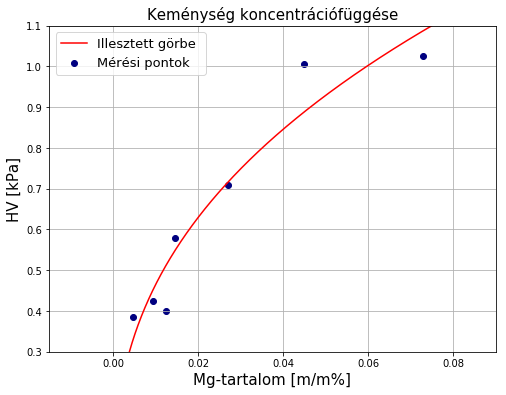
\includegraphics[scale=0.65]{szabad}
\caption{Minden paraméter illesztésével kapott görbe}
\label{fig:fit1}
\end{figure}
\newline
Az illesztési paraméterek:
\begin{gather*}
HV_0=(-0.062\pm 0.692) \hspace*{2pt}  \textrm{kPa}\\
B=(3.216\pm 1.487) \hspace*{2pt} \textrm{kPa}\\
m=0.393 \pm 0.379
\end{gather*}
Látszik, hogy az illesztési paraméterek hibája nagyon nagy, rendkívül bizonytalan az illesztés. Ebből az illesztésből sajnos következtetést ezért nem lehet levonni, ezért kötött kitevő, $m=1/2$ és $m=2/3$ esetére is elkészítettem az illesztést. Az így kapott illesztések a \ref{fig:fit2}. ábrán láthatók.\\
\begin{figure}[!h]
\centering
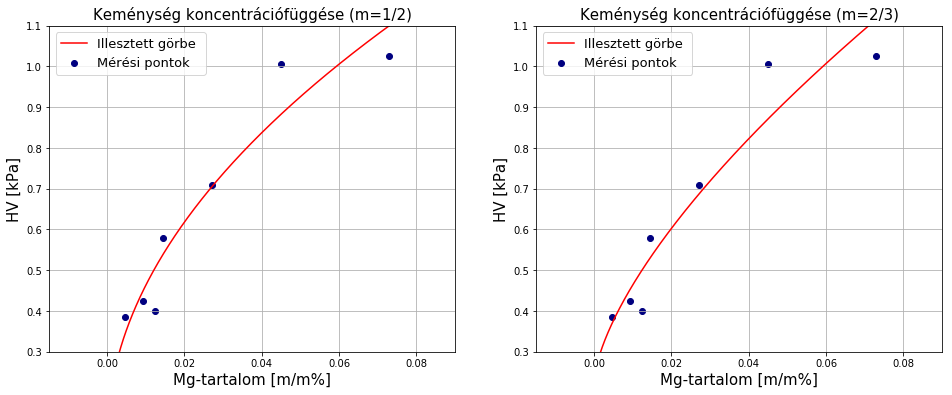
\includegraphics[scale=0.42]{illesztes}
\caption{A kitevő előre megválasztásával kapott illesztések}
\label{fig:fit2}
\end{figure}
\newline
Az illesztési paraméterek a két illesztés esetén:\\
\begin{table}[!h]
\begin{center}
\begin{tabular}{c c}
$m=1/2$ & $m=2/3$ \\
$HV_0=(0.089\pm 0.080) \hspace*{2pt}  \textrm{kPa}$ & $HV_0=(0.228\pm 0.068) \hspace*{2pt}  \textrm{kPa}$\\
$B=(3.741\pm 0.489) \hspace*{2pt} \textrm{kPa}$ & $B=(5.081\pm 0.709) \hspace*{2pt} \textrm{kPa}$\\
\end{tabular}
\end{center}
\end{table}
\newline
A paraméterek értékeiből és azok hibáiból jól látszik, hogy az $m=2/3$ esetben sokkal kisebb a relatív hiba, ezért mondhatjuk, hogy ez az eset írja le jobban az ötvözetet, vagyis az anyag már nem tekinthető egészen híg oldatnak, figyelembe kell venni az ötvözőatom-diszlokáció kölcsönhatásokat is.
\end{document}